\subsubsection{Indeterminate Structure Theory}
%Choose 2 truss designs and calculate the forces and deflections in the members using indeterminate structure theory (will be presented in class and tutorial Thursday May 20).

Structures three (figure \ref{fig:indeterm_3}) and five (figure \ref{fig:indeterm_5}) were analyzed using indeterminate structure theory. 
Tables \ref{tbl:indeterm_3} and \ref{tbl:indeterm_5} show the respective forces and deflections experienced by each member.
The applied load was assumed to be 1 N and the smallest Young's modulus (96 GPa) was used. %TODO: REWORD
The overall deflection in the third design (figure \ref{fig:indeterm_3}) was calculated to be 0.00558 mm, less than the 0.0107 mm predicted by the finite element analysis.
The overall deflection in the fifth design (figure \ref{fig:indeterm_5}) was seen to be 0.00554 mm, slightly greater than the 0.0036 mm predicted by the finite element analysis.

\begin{figure*}[p]
    \centering
    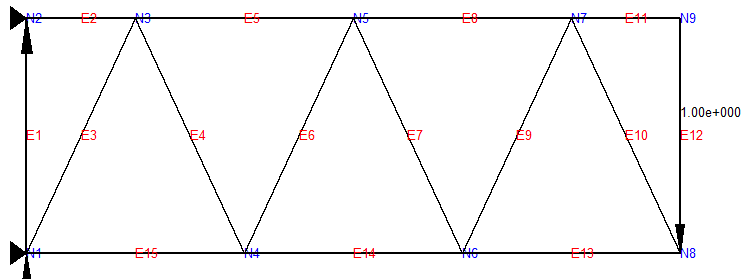
\includegraphics[width=0.8\textwidth]{images/truss3_given}
    \caption{Design Three}
    \label{fig:indeterm_3}
\end{figure*}

\begin{table*}[hp]
	\centering
	\caption{Design Three - Indeterminate Structures Analysis}
	\label{tbl:indeterm_3}
	\vspace{6pt}
	\begin{tabular}{ccc}
		\toprule
		Element & Force (N) & Element Deflection (m) \\
		\midrule
		1 & 1 & 6.578e-8 \\
		2 & 6 & 3.947e-7 \\ 
		3 & 1.4142  & 1.315e-7 \\ 
		4 & 1.4142  & 1.315e-7 \\ 
		5 & 4 & 5.2627e-7 \\ 
		6 & 1.4142  & 1.315e-7 \\ 
		7 & 1.4142 & 1.315e-7 \\ 
		8 & 2 & 2.63e-7 \\ 
		9 & 1.4142 & 1.315e-7 \\ 
		10 & 1.4142  & 1.315e-7 \\ 
		11 & 0 & 0 \\ 
		12 & 0  & 0 \\ 
		13 & 1  & 1.315e-7 \\ 
		14 & 3  & 3.947e-7 \\
		15 & 5 & 6.578e-7 \\
		\bottomrule
	\end{tabular}
\end{table*}

\begin{figure*}[p]
    \centering
    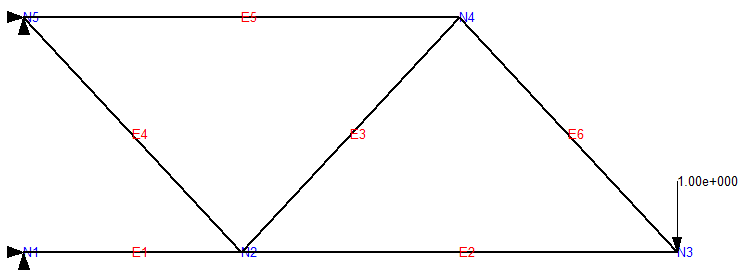
\includegraphics[width=0.8\textwidth]{images/truss5_given}
    \caption{Design Five}
    \label{fig:indeterm_5}
\end{figure*}

\begin{table*}[hp]
	\centering
	\caption{Design Five - Indeterminate Structures Analysis}
	\label{tbl:indeterm_5}
	\vspace{6pt}
	\begin{tabular}{ccc}
		\toprule
		Element & Force (N) & Element Deflection (m) \\
		\midrule
		1 &  -3 &  3.947e-7 \\
		2 &  -1 & 2.63e-7 \\
		3 &  -1.4142 &   2.60e-7 \\
		4 &  1.41421 &  2.63e-7 \\
		5 &  5 & 5.26e-7 \\
		6 &  1.41421 &  2.60e-7 \\ 
		\bottomrule
	\end{tabular}
\end{table*}